%!TEX TS-program = xelatex
%!TEX encoding = UTF-8 Unicode
%\documentclass[10pt, conference, compsocconf]{IEEEtran}
\documentclass{acm_proc_article-sp}
%\usepackage{fontspec}
%\usepackage{xunicode}
%\usepackage{xltxtra}
\usepackage{booktabs}
%\defaultfontfeatures{Mapping=tex-text}
%\setmainfont{Times New Roman}
%\usepackage{amsthm}
\usepackage{color}

\newcommand{\XXX}[1]{\textcolor{red}{{\it \textbf{[XXX: #1]}}}}


\usepackage{comment}
\newtheorem{mydef}{definition}
\usepackage{graphicx}
\newcommand{\slbl}[1]{\textbf{\textsf{#1}}}
\usepackage{multirow}%,multicolumn}
\usepackage{slashbox}
\usepackage{wrapfig}
\usepackage{booktabs, colortbl}
\usepackage{amsmath}
%\usepackage{amsmath,amssymb}
%\usepackage{algpseudocode}
%\usepackage[pdfstartview=FitH,xetex,bookmarksopenlevel=3,bookmarks=true]{hyperref}
% pdfpagescrop={92 112 523 778},
\usepackage[pdfstartview=FitH,bookmarksopenlevel=3,bookmarks=true]{hyperref} %pdfpagescrop={92 112 523 778},
%\usepackage{algorithm}%,algorithmic-fix}
\usepackage{url}
\begin{document}
\numberofauthors{5}
\author{
\alignauthor 
Abram Hindle\\
   \affaddr{David Cheriton School of Computer Science}\\
   \affaddr{University of Waterloo}\\
   \affaddr{Waterloo, Ontario, CANADA}\\
   \email{ahindle@uwaterloo.ca}
\alignauthor  Neil A. Ernst\\
   \affaddr{Department of Computer Science}\\
   \affaddr{University of Toronto}\\
   \affaddr{Toronto, Ontario, CANADA}\\
   \email{nernst@cs.toronto.edu}
\and
\alignauthor Michael W. Godfrey\\
   \affaddr{David Cheriton School of Computer Science}\\
   \affaddr{University of Waterloo}\\
   \affaddr{Waterloo, Ontario, CANADA}\\
   \email{migod@uwaterloo.ca}
\alignauthor Richard C. Holt \\
   \affaddr{David Cheriton School of Computer Science}\\
   \affaddr{University of Waterloo}\\
   \affaddr{Waterloo, Ontario, CANADA}\\
   \email{holt@uwaterloo.ca}
\alignauthor John Mylopoulos \\
   \affaddr{Department of Computer Science}\\
   \affaddr{University of Toronto}\\
   \affaddr{Toronto, Ontario, CANADA}\\
   \email{jm@cs.toronto.edu}}

\title{What's in a name? On the automated topic naming of software maintenance activities}

\maketitle
\thispagestyle{empty}

%There has not been any   investigation into the latent topics these %classifiers represent. 

\begin{abstract}

  

  Within the field of mining software repositories, many approaches,   such as topic modeling and concept location, rely on the automated   application of machine learning algorithms to corpora.  This kind of   approach typically makes no use of domain-specific knowledge to   improve the results or put them into a context that a developer can   relate to.  While too much specificity can produce non-generalizable   results, too little produces broad learners that do not provide much   immediately useful detail.  In this paper, we investigate what   topics the latent topic extractors produce, and examine whether   such topics can be generalized across software products.  We focus   on non-functional requirements related to software quality as a   potential generalization, since there is some shared belief that   these qualities apply broadly across many software systems and their   development artifacts.  In our approach, we name topics based on a   static ontology of non-functional requirements and software   qualities; in essence, this adds context to general-purpose   ontologies such as WordNet.  In this paper, we discuss how we use   this software development domain knowledge to better annotate topics   of development that are extracted from the change log messages in   configuration management systems such as CVS.  Since our taxonomy is   global in scope, our results allow us to compare the relative   importance of particular qualities across different projects. Within the topics extracted from MySQL and MaxDB we found that   non-functional requirements were common and often were trends across   time. Our automated techniques can label topics without much computational overhead.

\end{abstract}

\newcommand{\shrink}{}

\section{Introduction}
\begin{quote}
	\emph{What's in a name? that which we call a rose\\
	By any other name would smell as sweet;}
	\begin{flushright} -- Romeo and Juliet, II:ii\end{flushright}
\end{quote}

Few would argue that software development is a bed of roses.  To most of us, the important properties of a rose are sensual in nature, and concern appearance, odour, and feel.  While horticulturalists and botanists may see more semantic depth than this, one rose is often just as pleasing to us as another.  Software development artifacts, on the other hand, are abstract and intangible.  They are often unnamed and ephemeral --- even more so than roses --- and maybe partially derived from other unnamed and ephemeral artifacts.  Yet to have meaningful discussions about how software development is progressing, we must be able to devise appropriate labels for our work topics and be able to categorize the development artifacts as belonging to one or more of these topics. 

%Original is here:

%Unlike the poetic license Shakespeare uses, we show that names are
%indeed important. The rose has its own tangible properties which
%allow us to sense it. Unfortunately when we are dealing with data
%abstracted from program source code, we are already dealing with
%abstract entities that are not tangible.

% To have meaningful discussions about how software development is progressing, we must devise appropriate labels for our work topics, in contrast to the quote above. We can then categorize development artifacts as belonging to one or more of these topics. 


Topics arise from the wide variety of issues which occur during a software project's life-cycle. These topics can relate to, among others, the problem domain, the processes and tools used, or the development artifacts themselves.  The set of development topics for a given project can sometimes be extracted automatically by analyzing artifacts within software repositories, such as change-log comments that developers create when committing revisions to the project's source control system.  Our previous work dealt with topic trends, which are topics that recur over time~\cite{Hindle09ICSM}. We observed that topic trends were often non-functional requirements.


%As development of a software project progresses, developers must concern themselves with a wide variety of issues --- or ``topics'' --- that relate to the problem domain, the processes and tools used, the development artifacts themselves, etc.  The set of development topics for a given project can sometimes be extracted automatically by analyzing artifacts within software repositories, such as change-log comments that developers create when committing revisions to the project's source control system.  Our previous work dealt with topic trends, which are topics that recur over time~\cite{Hindle09ICSM}. We observed that topic trends were often non-functional requirements.

%During the development of a software project developers touch on many %issues integral to the purpose of the software project. These issues %are often referred to as topics. These topics can sometimes be %automatically extracted from the changelog comments that developers %create while committing revisions to the project's source control %repository. Our previous work dealt with %topic-trends~\cite{Hindle09ICSM}, topics that repeat overtime. It %seemed that these trends were often non-functional requirements. 

Topics in this paper and the previous paper are word bags or word distributions. These word distributions are found via Latent Dirichlet Allocation~\cite{Blei2003}, which finds independent word distributions shared among documents (change-log comments). The unfortunate aspect of topics that are word distributions is that they lack the tangibility of a rose. They do not self identify with their tangible properties. Topics have to be identified by interpreting the prevalent words in the word distribution and by inspecting related documents. This is impractical when one has to handle more than one hundred different topics. It would be nice if we could have automatic assistance to determine what the topic is about. This is the power of labelling and naming.


%If a topic has a name or a label we immediately have a good idea of  %what it is. In our case the name is the bit of information, the %summary, that was missing from our topics to make them useful and %complete. Although we are convinced that accurate naming is not %completely feasible, so we have focussed on labelling topics by %non-functional requirements.

A topic --- that is, a word distribution in our world --- needs a suggestive name to succinctly convey its intent, and make it easy to use in discussions and analyses about the development of the system. Our previous experience leads us to believe that automated topic naming is currently infeasible in the general case. We have therefore decided to focus on topic labels from the sub-domain of non-functional requirements related to software quality.

%In this paper we \textit{name} and \textit{label} topics generated by %a topic modeling technique, Latent Dirichlet %Allocation~\cite{Blei2003}. We use these topic models to train %supervised learners to classify larger datasets. We also show that %these topics can be generalized across products.

% Clean this up
Traditionally topic extraction has required manual annotation to derive domain-relevant labels. This paper attempts to implement \emph{labelled topic extraction}, in which topics are extracted and given labels relating to a cross-project taxonomy. This is an ontological approach where we attempt to relate networks of words to labels and then search for these terms within our topics. We also compare this approach to supervised machine learning.
%We start with an unsupervised topic learning algorithm, then manually %annotate the topics using the ontology. From the annotated topics, we %apply automated classifiers to find labels for the remaining topics. 

%\XXX{Not sure about this}
\begin{comment}
Typically what is distinct is the software's particular functionality -- whether it offers email composition, prepares tax returns, and so on. What is common, however, is the non-functional, or quality requirements, that the software focuses on. Our approach makes use of software quality taxonomies in order to compare different projects on similar concepts. For example, how is the Security quality treated over time by product A versus product B? Does product A care about it more as it matures? Does the quality occur more often in software commits?
\end{comment}

Our contributions include:
\begin{itemize}
\item  We introduce labelled topic extraction, and demonstrate its usefulness
  compared to other approaches.
% unsure about this
\item We show that these labels with their topics can be learnt and used to classify other data-sets.
\item We present visualizations of named topics and their trends over time to aid communication and analysis.
\item We use an exploratory case study of
  several open source database systems to show how named topics can be compared between projects.
\end{itemize}

We first introduce some important terminology for our work. We then describe our methodology, including our data-sets, then highlight our results. We conclude with a look at related work and possible improvements.

\shrink
\section{Background}

We provide a brief overview of software repository mining and information retrieval.
This work is related to the mining software repositories (MSR)~\cite{msr} research community as it deals expressly with analyzing a project's source control repository, and the messages associated with revisions therein.

\shrink
\subsection{Definitions}
We will use the following terminology in the rest of the paper.
A \emph{message} is a block of text written by a developer. In this
paper, messages will be the CVS and BitKeeper commit log comments made
when a developer commits changes to files in a repository. A \emph{word
  distribution} is the summary of a message by word count. Each word
distribution will be over the words in all messages. However, most
words will not appear in each message. A word distribution is effectively
a word count divided by the message size. A \emph{topic} is a word
distribution, i.e., a set of words that form a word distribution that is
unique and independent within the set of documents in our total
corpus. One could think of a topic as a distribution of the centroid
of a group of messages. In this paper we often summarize topics by the
top ten most frequent words of their word distribution.  A \emph{trend}
is one or more similar topics that recur over time.  Trends are
particularly important, as they indicate long-lived and recurring
topics that may provide key insights into the development of the
project. A \emph{label} is part of a title we attach to a topic, whether manually or automatically.

% area under the ROC 
% check
\emph{Area of ROC Curve} is the area under the Receiver Operating Characteristic (ROC) curve, sometimes referred to as \emph{AUC}. ROC values reflect a score, similar to school letter-grades (A is 0.9, C is 0.6), reflecting how well a particular learner performed for the given data. A ROC result of 0.5 would be equivalent to a random learner (randomly classifying data). ROC maps to the more familiar concepts of precision/sensitivity and recall/specificity: it plots the true positive rate (sensitivity) vs. the false positive rate (1 - specificity). A perfect learner has a ROC value of 1.0, reflecting perfect recall and precision.

\shrink
\subsection{Topic and Concept Extraction}
Topic extraction, sometimes called concept extraction, uses tools such as Latent Dirichlet Allocation (LDA)~\cite{Blei2003} and Latent Semantic Indexing (LSI) to extract
independent word distributions (topics) from
	documents (commit log comments). Many researchers~\cite{marcus04wcre,Poshyvanyk2007,lukins08wcre,Linstead2007} have applied tools like LSI and LDA for mining software repositories, in particular analyzing source code, bugs or developer comments.
\begin{comment}
Ideally these extracted topics 
correlate with actual development topics that the developers discussed
during the development of the software project. For example, our technique might identify a collection of words: ``list next has iterator add'', which we then identify (manually) as concerning the topics of collections and the Iterator pattern.
\end{comment}

Typically a topic analysis tool like LDA will try to find $N$ independent word distributions found within the word distributions of all the messages. Linear combinations of these $N$ word distributions are then meant to be able to recreate the word distributions of all of the underlying messages. These $N$ word distributions effectively form topics: cross cutting collections of words relevant to one or more documents. Our problem is that these topics are not easy to interpret, as the underlying pattern is not clear. We feel that automatic labelling or naming of these topics would be helpful with respect to interpreting the subject of a topic. LDA extracts topics in an unsupervised manner; the algorithm relies solely on the source data with no human intervention.

In topic analysis a single document, such as a commit message, can be related to multiple topics. Representing documents as a mixture of topics maps well to source code repository commits, which often have more than one purpose~\cite{Hindle09ICSM}.  A topic represents both a word distribution and a group of commit log comments that are related to each other by their content.  In this paper a topic is a set of tokens extracted from commit messages found within a project's source control system (SCS).

\begin{comment}
In this paper we use LDA to identify topics.  LDA works by creating topic models for each period. A topic model is a statistical summary of the important subjects for that data-set.  The input to the algorithm is a set of documents, with contents treated as a bag of words, and a parameter to set the number of topics to generate. The algorithm returns a word-document matrix relating the occurrence frequency of a 
 The idea is similar to other IR approaches like TF/IDF (term frequency/inverse document frequency), which find uncommon words that are not found in other word-lists. These approaches are unsupervised in that they rely solely on the source data with no human intervention.
\end{comment}

One issue that arises with use of unsupervised techniques is how to label the topics. While the topic models themselves are generated automatically, what to make of them is less clear. For example, in our previous work~\cite{Hindle09ICSM}, as well as in Baldi et al.~\cite{Baldi2008}, topics are named manually: human experts read the highest-frequency members of a topic and assign a keyword accordingly. E.g., for the word list \emph{``listener change remove add fire''}, Baldi et al. assign the keyword \emph{event-handling}. The labels are reasonable enough, but still require an expert in the field to determine them. Our technique is automated, because we match keywords from WordNet~\cite{Fellbaum1998} to words in the topic model. 

\shrink
\subsection{Supervised learning}
While unsupervised techniques (LSI and LDA are both unsupervised) are appealing in their lack of human intervention, and thus lower effort, supervised learners have the advantage of domain knowledge which typically means improved results. In supervised learning, the data is divided into slices. One slice is manually annotated by the domain expert, and the classifications he/she determines are applied to the remaining slices. In this paper, we employ the WEKA~\cite{weka09} and Mulan~\cite{mulan} machine learning frameworks in order to test supervised learning.


\shrink 
\section{Methodology}

\begin{comment}
% To gather the data, we first extract the commit log comments from a
% project's SCS repository. We filter out stop words and produce word distributions from these messages. These distributions are bucketed
% into 30-day non-overlapping windows. Each window is subject to LDA analysis. %Figure \ref{fig:commits}
% depicts the general process for processing and analyzing the commit messages.
\end{comment}


To evaluate our approach, we sought candidate systems that were
mature projects and had openly accessible source control repositories.
We also decided to select systems from the same application
domain, as we felt the functional requirements would probably be
broadly similar.
%We wanted to compare two mature software projects, that had open %repositories, within the same application domain. 
% This allows us to partially control for differences in functional %requirements. 
We selected MySQL and MaxDB as they were open-source, partially-commercial database systems. MaxDB started in the late 1970s as a research project, and was later acquired by SAP. As of version 7.500, released April 2007, the project has 940 thousand lines of C source code~\footnote{generated using David A. Wheeler's \emph{SLOCCount}.}.
%How many developers?
%There are approximately ... developers working on it. 
The MySQL project started in 1994 but MySQL 3.23 was released in early 2001. MySQL contains 320 thousand lines of C and C++ source code. 

\shrink
\subsection{Generating the data}
From each project, we used source control commit comments, the messages that programmers write when they commit revisions to a source control repository. We leveraged the data that we gathered in \cite{Hindle09ICSM} for this work. An example of a typical commit message is: \textit{``history annotate diffs bug fixed (if mysql\_real\_connect() failed there were two pointers to malloc'ed strings, with memory corruption on free(), of course)''}. We extracted these messages and indexed them by creation time. We summarized each message as a word distribution but removed stop-words such as common English words \emph{the} and \emph{at}.

From that data-set, we created an XML file which separated commits into
monthly windows. This size of period is smaller than the time between minor releases but large enough for there to be sufficient commits to analyze. We applied Blei's LDA implementation~\cite{Blei2003} against the word distributions of these commits, and generated list of topics per period. 
%A topic extracted in the first period Period 1, the most important %topic might have been ``security", with ``sql'' second, down on to %less relevant topics. 
We arbitrarily set the number of topics to generate to $20$, because past experimentation showed that fewer topics might aggregate multiple unique topics while any more topics seemed to dilute the results and create indistinct topics. As well, more than $20$ topics quickly became infeasible for inspection and it was difficult to discern the difference in topics.

\shrink
\subsection{Associating labels}
\begin{comment}
% We would like to `name' our topic models for each period. In this way, we can see how certain words -- subjects -- occur more or less often with each period.
\end{comment}

Topics are word distributions: essentially lists of words ranked by frequency, which can be burdensome to interpret and hard to distinguish and understand.
Once we had topics for each period, we tried to associate them with a label from a list of keywords and related terms. We performed simple string matching between these topics and our lists, `naming' a topic if it contained that word or words. We used several different word lists for comparison. 


Our first word list set, \textsf{exp1}, was generated using the ontology described in Kayed et al.~\cite{5072519}. That paper constructs an ontology for software quality measurement using eighty source documents, including research papers and international standards. The labels we used:
\begin{quotation}
\small \noindent \textsf{
integrity, security,
interoperability, testability, maintainability, traceability,
accuracy, modifiability, understandability, availability, modularity,
usability, correctness, performance, verifiability, efficiency,
portability, flexibility, reliability.
}
\end{quotation}

Our second word list set, \textsf{exp2}, relied on the ISO quality model (ISO9126)~\cite{iso9126}. ISO9126 describes six high-level quality requirements (listed in Table \ref{tbl:wnsig}). 
%There is some debate about the significance and importance of the %terms in this model. 
%However, it is ``an international standard and thus provides an %internationally accepted terminology for software quality \cite[p. %58]{Boegh2008},'' which is sufficient for the purposes of this %research. 
ISO9126 is ``an international standard and thus provides an internationally accepted terminology for software quality \cite[p. 58]{Boegh2008},'' that is sufficient for the purposes of this research.
However, the terms extracted from ISO9126 may not capture all words associated with the labels.  For example, the term ``redundancy'' is one most would agree is relevant to discussion of reliability, but is not in the standard. We therefore took the words from the taxonomy and expanded them.

%Cite mockus et al

To construct these expanded word-lists, we used WordNet~\cite{Fellbaum1998}, an English-language ``lexical database'' that contains semantic relations between words, including meronymy and synonymy. We then added Boehm’s 1976 software quality model \cite{Boehm+:1976:ICSE}, and classified his eleven ‘ilities’ into their respective ISO9126 qualities. We did the same for the quality model produced by McCall et al. \cite{mccall1977}. Finally, we analyzed two mailing lists from the KDE project to enhance the specificity of the sets. We selected KDE-Usability, which focuses on usability discussions for KDE as a whole; and KDE-Konqueror, a list about a long-lived web browser project. For each high-level quality in ISO9126, we first searched for our existing labels; we then randomly sampled twenty-five mail messages that were relevant to that quality, and selected co-occurring terms relevant to that quality. For example, we add the term ``performance'' to the synonyms for \emph{efficiency}, since this term occurs in most KDE mail messages that discuss efficiency.
%exp2

For the third -- \textsf{exp3} -- list of quality labels, we extended the list from \textsf{exp2} using unfiltered WordNet similarity matches. Similarity in WordNet means siblings in a hypernym tree. We do not include these words here for space considerations (but see the Appendix for our data repository). It is not clear the words associated with our labels are specific enough, however: for example, the label \emph{maintainability} is associated with words \emph{ease} and \emph{ownership}.

\begin{table*}
	\centering
\begin{tabular}{c|p{9cm}}
\toprule
\textbf{Label} & \textbf{Related terms} \\
\midrule
\emph{Maintainability} &
testability changeability analyzability stability maintain maintainable modularity modifiability understandability + interdependent dependency encapsulation decentralized modular\\ \hline
\emph{Functionality} &
security compliance accuracy interoperability suitability functional practicality functionality + compliant exploit certificate secured “buffer overflow” policy malicious trustworthy vulnerable vulnerability accurate secure vulnerability correctness accuracy\\ \hline
\emph{Portability} &
conformance adaptability replaceability installability portable movableness movability portability + specification migration standardized l10n localization i18n internationalization documentation interoperability transferability\\ \hline
\emph{Efficiency} &
“resource behaviour” “time behaviour” efficient efficiency + performance profiled optimize sluggish factor penalty slower faster slow fast optimization\\ \hline
\emph{Usability} &
operability understandability learnability useable usable serviceable usefulness utility useableness usableness serviceableness serviceability usability + gui accessibility menu configure convention standard feature focus ui mouse icons ugly dialog guidelines click default human convention friendly user screen interface flexibility\\ \hline
\emph{Reliability} &
“fault tolerance” recoverability maturity reliable dependable responsibleness responsibility reliableness reliability dependableness dependability + resilience integrity stability stable crash bug fails redundancy error failure\\ 
\bottomrule
\end{tabular}
	\caption{Qualities and associated signifiers – WordNet version (\textsf{exp2})}
	\label{tbl:wnsig}

\end{table*}

\shrink
\subsection{Supervised learning}

\label{sec:suplearn}

In order to validate how effective these word-bag approaches to topic labelling would be we had to make a data set to test against.  For MySQL 3.23 and MaxDB 7.500, we manually annotated each extracted topic in each period with the same quality labels as \textsf{exp2} (software qualities). We looked at each period's topics, and assessed what the data -- consisting of the frequency-weighted word lists and messages -- suggested was the topic for that period. We were able to pinpoint the appropriate label using auxiliary information as well, such as the actual revisions and files that were related to this topic. For example, for the MaxDB topic consisting of a message ``exit() only used in non NPTL LINUX Versions'', we tagged that topic \emph{portability}. We compared against this data-set, but we also used it for our supervised learning based topic classification.
%inter-rater reliability 

We first compared our previous analysis using label matching to our manual classifications to get an error rate for that process described below in Section \ref{sec:unsuplabelling}. 

For supervised learning, we used a suite of supervised classifiers from WEKA~\cite{weka09}. WEKA contains a suite of machine learning tools such as support vector machines and Bayes nets. We also used the multi-labelling add-on for WEKA, Mulan~\cite{mulan}\footnote{\url{http://mlkd.csd.auth.gr/multilabel.html}}. Traditional classifiers map our topics to a single class, whereas Mulan allows for a mixture of classes per topic, which maps to what we observed while manually labelling topics.

To assess the performance of the supervised learners, we did a 10-fold cross-validation. This is when a set is partitioned into 10 partitions and then each partition is used once as a test set and 9 other times as part of the training set of 9 partitions. We have reported these results below in Section \ref{sec:suplabelling}.

Finally, using this data, we evaluated two research questions (see
Section \ref{sec:comparison}):
\begin{enumerate}
\item Do label frequencies change over time? That is, is a certain quality of more interest at one point in the life-cycle than some other? 
\item  Do the different projects differ in their relative topic interest? That is, is a particular quality more important to one project than the other projects?  
\end{enumerate}

\shrink
\section{Observations and evaluation}

\shrink
\subsection{Word list similarity}

% word list similarity

In general, this approach did not work out well as common labels
dominated the less common labels. The related words for
\emph{correctness}, for example, tended to be too lengthy and
non-specific. 
Table \ref{tbl:wordlist} lists results. 
A \emph{named   topic} is a topic with a matching label. There are \{periods X 20\} topics per project as we told LDA to extract 20 topics per period. All experiments were run on MaxDB 7.500 and MySQL 3.23 data.

%\begin{comment}
%\XXX{this table should have mysql}
\begin{table}
	\centering
\begin{tabular}{c|c|c|c}
\toprule
Measure &		 \textsf{exp1} &	 \textsf{exp2} &	 \textsf{exp3} \\
\midrule
Topics &			500		 &			500  	 & 		500  \\
Named topics &		281      &			125      &		328  \\
Unnamed topics &	139      &			295      &      92   \\
\bottomrule
\end{tabular}
	\caption{Automatic topic labelling for MaxDB 7.500}
	\label{tbl:wordlist}

\end{table}
%\end{comment}
%This is the counts

For \textsf{exp1}, our best performing labels (the labels matched with the most topics) were \emph{correctness} (182 topics) and \emph{testability} (121). We did not get good results for usability or accuracy, which were associated with fewer than ten topics. We also looked for correlation between our labels: Excluding double matches (self-correlation), our highest co-occurring terms were verifiability and traceability, and testability and correctness (76 and 62 matches, respectively).

For \textsf{exp2}, there are many more unnamed topics. Only reliability produces a lot of matches, mostly with the word `error'. Co-occurrence results were poor.

For \textsf{exp3}, we had many more named topics. As we mentioned, the word-lists are quite broad, so there are likely to be false-positives. See the following sections for our error analysis. We found a high of 265 topics for usability, with a low of 44 topics for maintainability. Common co-occurrences were reliability and usability, efficiency and reliability, and efficiency and usability (200, 190, and 150 topics in common, respectively). 

\shrink
\subsection{Analysis of the unsupervised labelling}

\label{sec:unsuplabelling}

Based on the labels, and our manual topic labelling, we compared the results of the unsupervised word matching approach. For each quality we tried to assess whether the manual tag matched the unsupervised label assigned. Table \ref{tbl:maxdb-unsup-results} shows our results for MaxDB and MySQL. In general results are poor. Using the F-Measure, the weighted average of precision and recall, where 1 is perfect, our best results are 0.6, a few at 0.4, and most around 0.2. We achieved similar results using the Matthew's correlation coefficient (used to measure efficacy where classes are of different sizes) and ROC.  

\begin{table*}%[ht]
	\centering

\begin{tabular}{c|c|c|c|c|c|c}
\toprule
Experiment & Label & F1 & MCC & Precision & Recall & ROC  \\ 
\midrule
MaxDB exp2 & portability & 0.228 & 0.182 & 0.520 & 0.146 & 0.553 \\ 
 & efficiency & 0.217 & 0.125 & 0.237 & 0.200 & 0.558\\ 
 & reliability & 0.380 & 0.340 & 0.246 & 0.829 & 0.765 \\ 
 & functionality & 0.095 & 0.083 & 0.250 & 0.059 & 0.521 \\ 
 & maintainability & 0.092 & 0.123 & 0.571 & 0.050 & 0.520 \\ 
 & usability & 0.175 & 0.138 & 0.113 & 0.389 & 0.620 \\ 
 & total & 0.236 & 0.127 & 0.248 & 0.225 & 0.561 \\ 
\midrule
MySQL exp2 & portability & 0.138 & 0.211 & 1.000 & 0.074 & 0.537 \\ 
 & efficiency & 0.345 & 0.327 & 0.476 & 0.270 & 0.625 \\ 
 & reliability & 0.425 & 0.287 & 0.348 & 0.545 & 0.669 \\ 
 & functionality & 0.025 & 0.006 & 0.571 & 0.013 & 0.501 \\ 
 & maintainability & 0.000 & 0.000 & 0.000 & 0.000 & 0.500 \\ 
 & usability & 0.175 & 0.135 & 0.200 & 0.156 & 0.560 \\ 
 & total & 0.167 & 0.095 & 0.403 & 0.105 & 0.527 \\ 
\midrule
MaxDB exp3 & portability & 0.472 & 0.286 & 0.402 & 0.573 & 0.660 \\ 
 & efficiency & 0.223 & 0.068 & 0.130 & 0.778 & 0.549 \\ 
 & reliability & 0.257 & 0.196 & 0.149 & 0.927 & 0.652 \\ 
 & functionality & 0.236 & 0.187 & 0.138 & 0.824 & 0.665 \\ 
 & maintainability & 0.338 & 0.112 & 0.266 & 0.463 & 0.566 \\ 
 & usability & 0.108 & 0.094 & 0.057 & 0.944 & 0.595 \\ 
 & total & 0.258 & 0.093 & 0.160 & 0.671 & 0.568 \\ 
\midrule
MySQL exp3 & portability & 0.413 & 0.170 & 0.564 & 0.325 & 0.574 \\ 
 & efficiency & 0.158 & 0.105 & 0.089 & 0.703 & 0.608 \\ 
 & reliability & 0.388 & 0.240 & 0.260 & 0.758 & 0.660 \\ 
 & functionality & 0.652 & 0.240 & 0.655 & 0.649 & 0.620 \\ 
 & maintainability & 0.203 & 0.007 & 0.240 & 0.175 & 0.503 \\ 
 & usability & 0.105 & 0.013 & 0.057 & 0.688 & 0.513 \\ 
 & total & 0.362 & 0.076 & 0.284 & 0.499 & 0.544 \\
\bottomrule
\end{tabular}
	\caption{Results for automatic topic labelling. F1 = f-measure, MCC = Matthew's correlation coeff., ROC = Area under ROC curve}
	\label{tbl:maxdb-unsup-results}
\end{table*}

Based on these results we find that reliability and usability worked well for MaxDB in \textsf{exp2} and better in \textsf{exp3}. MySQL had reasonable results within \textsf{exp2} for reliability and efficiency. MySQL's results for efficiency did not improve in \textsf{exp3} but other qualities such as functionality did improve. If a \emph{C} grade performance has a ROC value of $0.6$ then most of these tests scored \emph{C} or less, but our results were still better than random chance.

%\subsection{Classifying topics}
\shrink
\subsection{Analysis of the supervised labelling}
\label{sec:suplabelling}

We took our annotated data-set and applied supervised learners to it. Because our data-set was of word counts we expected Bayesian techniques, often used in spam filtering, to perform well. We also tried other learners that WEKA~\cite{weka09} provides: rule learners, tree learners, vector space learners, and support vector machines.  Table \ref{tab:best-learn-per-tag} shows the performance of the best performing learner per label.  We considered the best learner for a label to be the one which had the highest ROC value for that label. Table \ref{tab:best-learn-per-tag} uses the ZeroR learner as a baseline, since it naively chooses the largest category all of the time. The ZeroR difference is often negative. For labels which are not as common, this can be expected because any miscategorization will hurt accuracy. This is why the F1 (F-measure) and the ROC values are useful, as they can better present performance on labels which are not applicable to the majority of samples.

Table \ref{tab:best-learn-per-tag} shows that MaxDB and MySQL have quite different results, as the ROC values for reliability and functionality seem swapped between projects. It should be noted that for both projects Bayesian techniques did the best out of a wide variety of machine learners tested. Discriminative Multinomial Naive Bayes (DMNBtext), Naive Bayes (NaiveBayes) and Multinomial Naive Bayes (NaiveBayesMultinomal) are all based on Bayes's theorem and all assume, naively, that the features are independent. The features we used are word counts per message. One beneficial aspect of this result is that it suggests we can have very fast training and classifying  since Naive Bayes can be calculated in $O(N)$ for $N$ features.
%http://nlp.stanford.edu/IR-book/html/htmledition/naive-bayes-text-classification-1.html

The smaller the label the harder it is to get accurate results. Nevertheless, these results are better than our previous word bag results of \textsf{exp2} and \textsf{exp3}, because the ROC values are sufficiently higher in most cases (other than MaxDB reliability and MySQL efficiency).

The limitation of the approach we took here is that we assume labels are independent; however, labels could be correlated with each other. We also did not evaluate how well the learners performed together.


% Cribbed from: 
% src/validate/latex-out/best-learner-per-project-roc-table.txt
\begin{table*}
\centering
\begin{tabular}{ccc|rrrr}
\toprule
Label & Project & Learner & ROC & ZeroR Acc. & ZeroR. Diff & F1\\
\midrule

portability &  MySQL &  NaiveBayesMultinomial &  0.74 &  58.53 &  11.43 &  0.62 \\
efficiency &  MySQL &  NaiveBayes &  0.67 &  93.69 &  -7.68 &  0.23 \\ 
reliability &  MySQL &  NaiveBayes &  0.73 &  83.11 &  -12.80 &  0.41 \\ 
functionality &  MySQL &  DMNBtext &  0.81 &  54.44 &  21.67 &  0.77  \\ 
maintainability &  MySQL &  DMNBtext &  0.78 &  76.62 &  3.41 &  0.32  \\ 
usability &  MySQL &  NaiveBayes &  0.75 &  94.54 &  -5.80 &  0.21  \\ 
 \hline 
portability &  MaxDB &  NaiveBayes &  0.84 &  77.12 &  2.06 &  0.61 \\ 
efficiency &  MaxDB &  NaiveBayes &  0.62 &  88.43 &  -11.31 &  0.25  \\ 
reliability &  MaxDB &  DMNBtext &  0.84 &  89.46 &  3.86 &  0.57  \\ 
functionality &  MaxDB &  NaiveBayes &  0.67 &  91.26 &  -6.94 &  0.31  \\ 
maintainability &  MaxDB &  NaiveBayes &  0.70 &  79.43 &  -9.25 &  0.42  \\ 
usability &  MaxDB &  NaiveBayes &  0.56 &  95.37 &  -4.37 &  0.00  \\ 
 \hline 


% this was before I fixed an fmeasure bug
% 
% portability &  MySQL &  NaiveBayesMultinomial &  0.74 &  58.53 &  11.43 &  0.70  \\ 
% efficiency &  MySQL &  NaiveBayes &  0.67 &  93.69 &  -7.68 &  0.88 \\ 
% reliability &  MySQL &  NaiveBayes &  0.73 &  83.11 &  -12.80 &  0.74 \\ 
% functionality &  MySQL &  DMNBtext &  0.81 &  54.44 &  21.67 &  0.76 \\ 
% maintainability &  MySQL &  DMNBtext &  0.78 &  76.62 &  3.41 &  0.75 \\ 
% usability &  MySQL &  NaiveBayes &  0.75 &  94.54 &  -5.80 &  0.90  \\ 
% %total & MySQL & NaibeBayes & 0.75 & 
%  \hline 
% portability &  MaxDB &  NaiveBayes &  0.84 &  77.12 &  2.06 &  0.80 \\ 
% efficiency &  MaxDB &  NaiveBayes &  0.62 &  88.43 &  -11.31 &  0.79 \\ 
% reliability &  MaxDB &  DMNBtext &  0.84 &  89.46 &  3.86 &  0.92  \\ 
% functionality &  MaxDB &  NaiveBayes &  0.67 &  91.26 &  -6.94 &  0.86  \\ 
% maintainability &  MaxDB &  NaiveBayes &  0.70 &  79.43 &  -9.25 &  0.72  \\ 
% usability &  MaxDB &  NaiveBayes &  0.56 &  95.37 &  -4.37 &  0.91  \\ 

\end{tabular}
\caption{Per label, per project, the best learner for that label. ROC value rates learner performance, compared with the ZeroR learner ( a learner which just chooses the largest category all of the time). F1 is the F-measure for that particular learner.}
\label{tab:best-learn-per-tag}
\end{table*}


\shrink
\subsection{Applying multiple labels to topics}

We applied the Mulan~\cite{mulan} library for Multi-Label learning to our data-set because intuitively, topics can have more than one label, much like how a particular source code revision can have more than one topic. Multi-label learning is more than just classifying entities with more than one label. It also includes methods for determining the performance of such techniques. The problem framed in the learners above has changed; instead of looking at the precision and recall of applying one label, we rank multiple labels at once. We must check if the full subset of labels was applied, and then how much of that subset was applied.

Another aspect of multi-label learning are micro versus macro measurements. Macro measurements are aggregated at a class or label level. Micro measurements are aggregated at a decision level. So a macro-ROC measurement is the average ROC over the ROC values for all labels, where a micro-ROC is the average ROC over all examples that were classified. Unfortunately for MaxDB, the macro-ROC values are undefined because of poor performance of one of the labels.

We have presented the results of Mulan's multi-label learners in Table \ref{tab:mulan}.  Binary Relevance (BR), Calibrated Label Ranking (CLR) and Hierarchy Of Multi-label classifiERs (HOMER), performed the best. HOMER and BR act as a hierarchy of learners: BR is flat, while HOMER tries to build a deeper hierarchy to build a more accurate learner~\cite{mulan}. These classifiers performed better than other multi-label classifiers. They have the best micro and macro ROC scores, although their results seem comparable to the naive Bayesian learners we used in Section \ref{sec:suplabelling}.

\begin{comment}

\begin{table*}
\centering
\begin{tabular}{l|rrrrrrrr}

  & BR & CLR & HOMER & IncludeLabels & LP & MLStacking & MLkNN & RAkEL \\

\hline \\

example Accuracy & 0.45 & 0.40 & 0.50 & 0.40 & 0.40 & 0.38 & 0.33 & 0.48 \\

example F1 & 0.56 & 0.48 & 0.59 & 0.47 & 0.49 & 0.46 & 0.40 & 0.55 \\

% example Hamming loss & 0.24 & 0.19 & 0.18 & 0.19 & 0.23 & 0.19 & 0.20 & 0.17 \\

example Precision & 0.50 & 0.51 & 0.60 & 0.52 & 0.52 & 0.50 & 0.44 & 0.60 \\

example Recall & 0.65 & 0.46 & 0.58 & 0.44 & 0.47 & 0.43 & 0.37 & 0.52 \\

example Subset Accuracy & 0.19 & 0.24 & 0.31 & 0.24 & 0.23 & 0.23 & 0.20 & 0.31 \\

label macro-ROC & 0.74 & 0.66 & 0.64 & 0.60 & 0.56 & 0.58 & 0.59 & 0.67 \\

label macro-F1 & 0.46 & 0.30 & 0.43 & 0.28 & 0.32 & 0.27 & 0.22 & 0.39 \\

label macro-Precision & 0.41 & 0.41 & 0.49 & 0.39 & 0.37 & 0.34 & 0.34 & 0.52 \\

label macro-Recall & 0.56 & 0.26 & 0.40 & 0.24 & 0.31 & 0.23 & 0.19 & 0.33 \\

label micro-ROC & 0.81 & 0.81 & 0.77 & 0.77 & 0.66 & 0.80 & 0.80 & 0.79 \\

label micro-F1 & 0.59 & 0.53 & 0.61 & 0.51 & 0.50 & 0.51 & 0.45 & 0.59 \\

label micro-Precision & 0.51 & 0.69 & 0.66 & 0.71 & 0.53 & 0.70 & 0.69 & 0.73 \\

label micro-Recall & 0.68 & 0.43 & 0.56 & 0.41 & 0.48 & 0.41 & 0.34 & 0.49 \\

% rank Avg. Precision & 0.76 & 0.77 & 0.69 & 0.72 & 0.53 & 0.74 & 0.76 & 0.73 \\

% rank Coverage & 1.51 & 1.47 & 1.94 & 1.72 & 2.99 & 1.57 & 1.54 & 2.00 \\

% rank One-error & 0.40 & 0.39 & 0.47 & 0.44 & 0.63 & 0.43 & 0.40 & 0.36 \\

% rank Ranking Loss & 0.19 & 0.18 & 0.27 & 0.22 & 0.52 & 0.20 & 0.19 & 0.28 \\

\end{tabular}
\caption{Mysql Mulan results per Mulan learner}
\end{table*}


\begin{table*}
% Cribbed from:
% src/validate/output/maxdb.mulan.out.tex
\centering
\begin{tabular}{l|rrrrrrrr}

  & BR & CLR & HOMER & IncludeLabels & LP & MLStacking & MLkNN & RAkEL \\

\hline \\

example-Accuracy & 0.49 & 0.47 & 0.51 & 0.44 & 0.42 & 0.47 & 0.43 & 0.48 \\

example-Fmeasure & 0.55 & 0.50 & 0.53 & 0.45 & 0.44 & 0.48 & 0.43 & 0.50 \\

example-HammingLoss & 0.19 & 0.14 & 0.14 & 0.14 & 0.17 & 0.13 & 0.13 & 0.13 \\

example-Precision & 0.50 & 0.49 & 0.53 & 0.45 & 0.45 & 0.49 & 0.43 & 0.51 \\

example-Recall & 0.61 & 0.50 & 0.53 & 0.45 & 0.43 & 0.47 & 0.43 & 0.50 \\

example-SubsetAccuracy & 0.40 & 0.43 & 0.45 & 0.43 & 0.38 & 0.43 & 0.43 & 0.43 \\

label-macro-AUC & NaN & NaN & NaN & NaN & NaN & NaN & NaN & NaN \\

label-macro-F1 & 0.32 & 0.19 & 0.23 & 0.11 & 0.19 & 0.12 & 0.00 & 0.26 \\

label-macro-Precision & 0.29 & 0.31 & 0.32 & 0.21 & 0.23 & 0.18 & 0.00 & 0.40 \\

label-macro-Recall & 0.38 & 0.15 & 0.20 & 0.08 & 0.17 & 0.10 & 0.00 & 0.23 \\

label-micro-AUC & 0.76 & 0.66 & 0.62 & 0.55 & 0.62 & 0.68 & 0.65 & 0.68 \\

label-micro-F1 & 0.39 & 0.27 & 0.34 & 0.13 & 0.25 & 0.21 & 0.00 & 0.34 \\

label-micro-Precision & 0.34 & 0.42 & 0.49 & 0.33 & 0.30 & 0.49 & 0.00 & 0.49 \\

label-micro-Recall & 0.47 & 0.21 & 0.26 & 0.09 & 0.22 & 0.14 & 0.00 & 0.27 \\

rank-AvgPrecision & 0.54 & 0.57 & 0.54 & 0.40 & 0.40 & 0.60 & 0.58 & 0.51 \\

rank-Coverage & 1.40 & 1.23 & 1.43 & 1.84 & 1.93 & 1.16 & 1.20 & 1.54 \\

rank-One-error & 0.81 & 0.79 & 0.81 & 0.90 & 0.89 & 0.76 & 0.79 & 0.79 \\

rank-Ranking Loss & 0.41 & 0.35 & 0.41 & 0.58 & 0.60 & 0.32 & 0.33 & 0.46 \\

\end{tabular}

\caption{Maxdb Mulan results per Mulan learner}

\end{table*}

\end{comment}


\begin{table*}%[h]
\centering
\begin{tabular}{l|ccc|ccc}
\toprule
  & MySQL & MySQL & MySQL &                         MaxDB & MaxDB & MaxDB  \\ 
Performance Metric  & BR & CLR & HOMER &                              BR & CLR & HOMER \\      

\midrule
%\hline \\

% example Accuracy & 0.45 & 0.40 & 0.50 &           0.49  &  0.47  &  0.51 \\ 
                                                                            
% example F1 & 0.56 & 0.48 & 0.59 &           0.55  &  0.50  &  0.53 \\ 
                                                                            
% example Hamming Loss & 0.24 & 0.19 & 0.18 &        0.19  &  0.14  &  0.14 \\ 
                                                                            
% example Precision & 0.50 & 0.51 & 0.60 &          0.50  &  0.49  &  0.53 \\ 
                                                                            
% example Recall & 0.65 & 0.46 & 0.58 &             0.61  &  0.50  &  0.53 \\ 
                                                                            
example Subset Accuracy & 0.19 & 0.24 & 0.31 &     0.40  &  0.43  &  0.45 \\ 
      \hline                                                                      
label macro-ROC & 0.74 & 0.66 & 0.64 &            NaN  &  NaN  &  NaN    \\ 
                                                                            
label macro-F1 & 0.46 & 0.30 & 0.43 &             0.32  &  0.19  &  0.23 \\ 
                                                                            
label macro-Precision & 0.41 & 0.41 & 0.49 &      0.29  &  0.31  &  0.32 \\ 
                                                                            
label macro-Recall & 0.56 & 0.26 & 0.40 &         0.38  &  0.15  &  0.20 \\ 
                                                                            
label micro-ROC & 0.81 & 0.81 & 0.77 &            0.76  &  0.66  &  0.62 \\ 
                                                                            
label micro-F1 & 0.59 & 0.53 & 0.61 &             0.39  &  0.27  &  0.34 \\ 
                                                                            
label micro-Precision & 0.51 & 0.69 & 0.66 &      0.34  &  0.42  &  0.49 \\ 
                                                                            
label micro-Recall & 0.68 & 0.43 & 0.56 &         0.47  &  0.21  &  0.26 \\ 
       \hline                                                                      
 rank Avg. Precision & 0.76 & 0.77 & 0.69 &          0.54  &  0.57  &  0.54 \\ 
                                                                            
 rank Coverage & 1.51 & 1.47 & 1.94 &              1.40  &  1.23  &  1.43 \\ 
                                                                            
 rank One-error & 0.40 & 0.39 & 0.47 &             0.81  &  0.79  &  0.81 \\ 
                                                                            
 rank Ranking Loss & 0.19 & 0.18 & 0.27 &          0.41  &  0.35  &  0.41 \\ 
\hline
\end{tabular}
\caption{MySQL and MaxDB Mulan results per Multi-Label learner}
\label{tab:mulan}
\end{table*}

\shrink
\subsection{Summary of techniques}

Very rarely did \textsf{exp2} and \textsf{exp3} (naive word matching) ever perform as well as the machine learners. For MaxDB, reliability was slightly better detected using the static word list of \textsf{exp2}. In general, the machine learners and \textsf{exp3} did better than \textsf{exp2} for both MaxDB and MySQL. For both MySQL and MaxDB usability was better served by \textsf{exp2}. Usability was a very infrequent label, however.

We found that the multi-label learners of BR, CLR and HOMER did not do as well for Macro-ROC and Micro-F1 as NaiveBayes and other NaiveBayes derived learners did. This suggests that by sticking together multiple NaiveBayes learners we could probably label topics effectively, but it would require a separate NaiveBayes learner per label.

\begin{comment}
MySQL Macro ROC 0.746 Micro F1 0.78 Mulan BR ROC 0.74 / 0.81 F1 0.46/0.59/0.56 
MaxDB Macro ROC 0.7   Micro F1 0.83 Mulan BR ROC NaN  / 0.76 F1 0.32/0.39/0.55

\end{comment}


\begin{comment}
           exp2 exp3 learn  B 2nd
maxdb port 0.55 0.66 0.74   L 3
maxdb eff  0.55 0.64 0.67   L 3
maxdb rel  0.76 0.65 0.73   2 2
maxdb fun  0.52 0.66 0.81   L 3
maxdb main 0.52 0.56 0.78   L 3
maxdb use  0.62 0.59 0.75   L 2

mysql port 0.53 0.57 0.85   L 3
mysql eff  0.62 0.60 0.62   2 2 
mysql rel  0.66 0.66 0.84   L 3
mysql fun  0.5  0.62 0.67   L 3
mysql main 0.5  0.5  0.70   L 3
mysql use  0.56 0.51 0.56   L 2
\end{comment}

\shrink
\subsection{Visualization}

We have created two visualizations of the manually labelled data. A problem we faced while visualizing was how to display tag overlaps. Our solution, while not optimal, was to assign a separate colour to each distinct set of annotations. Figures \ref{fig:maxdb} and \ref{fig:mysql} show extracted topics grouped by annotations. Annotations or labels that occur in adjacent windows are joined together as trends. For MaxDB (Figure \ref{fig:maxdb}) the largest trends were related to maintainability and portability. MaxDB supports numerous platforms and portability was a constant issue facing the project's development. MySQL was different, with many topics overlapping, so there were many different subsets. Functionality trends were prevalent throughout its history (the largest reddish streak across the top). Two combination  tags of ``functionality portability'' (orange) and ``maintainability portability'' (teal) streaked across most of the history of MySQL. Since this was MySQL 3.23, a stable branch, we expect that issues dealing with portability and maintenance would be the primary concerns of this branch: developers probably wanted it to work with current systems and thus had to update it.

\begin{figure*}
  \centering
  % hi-res version
  % 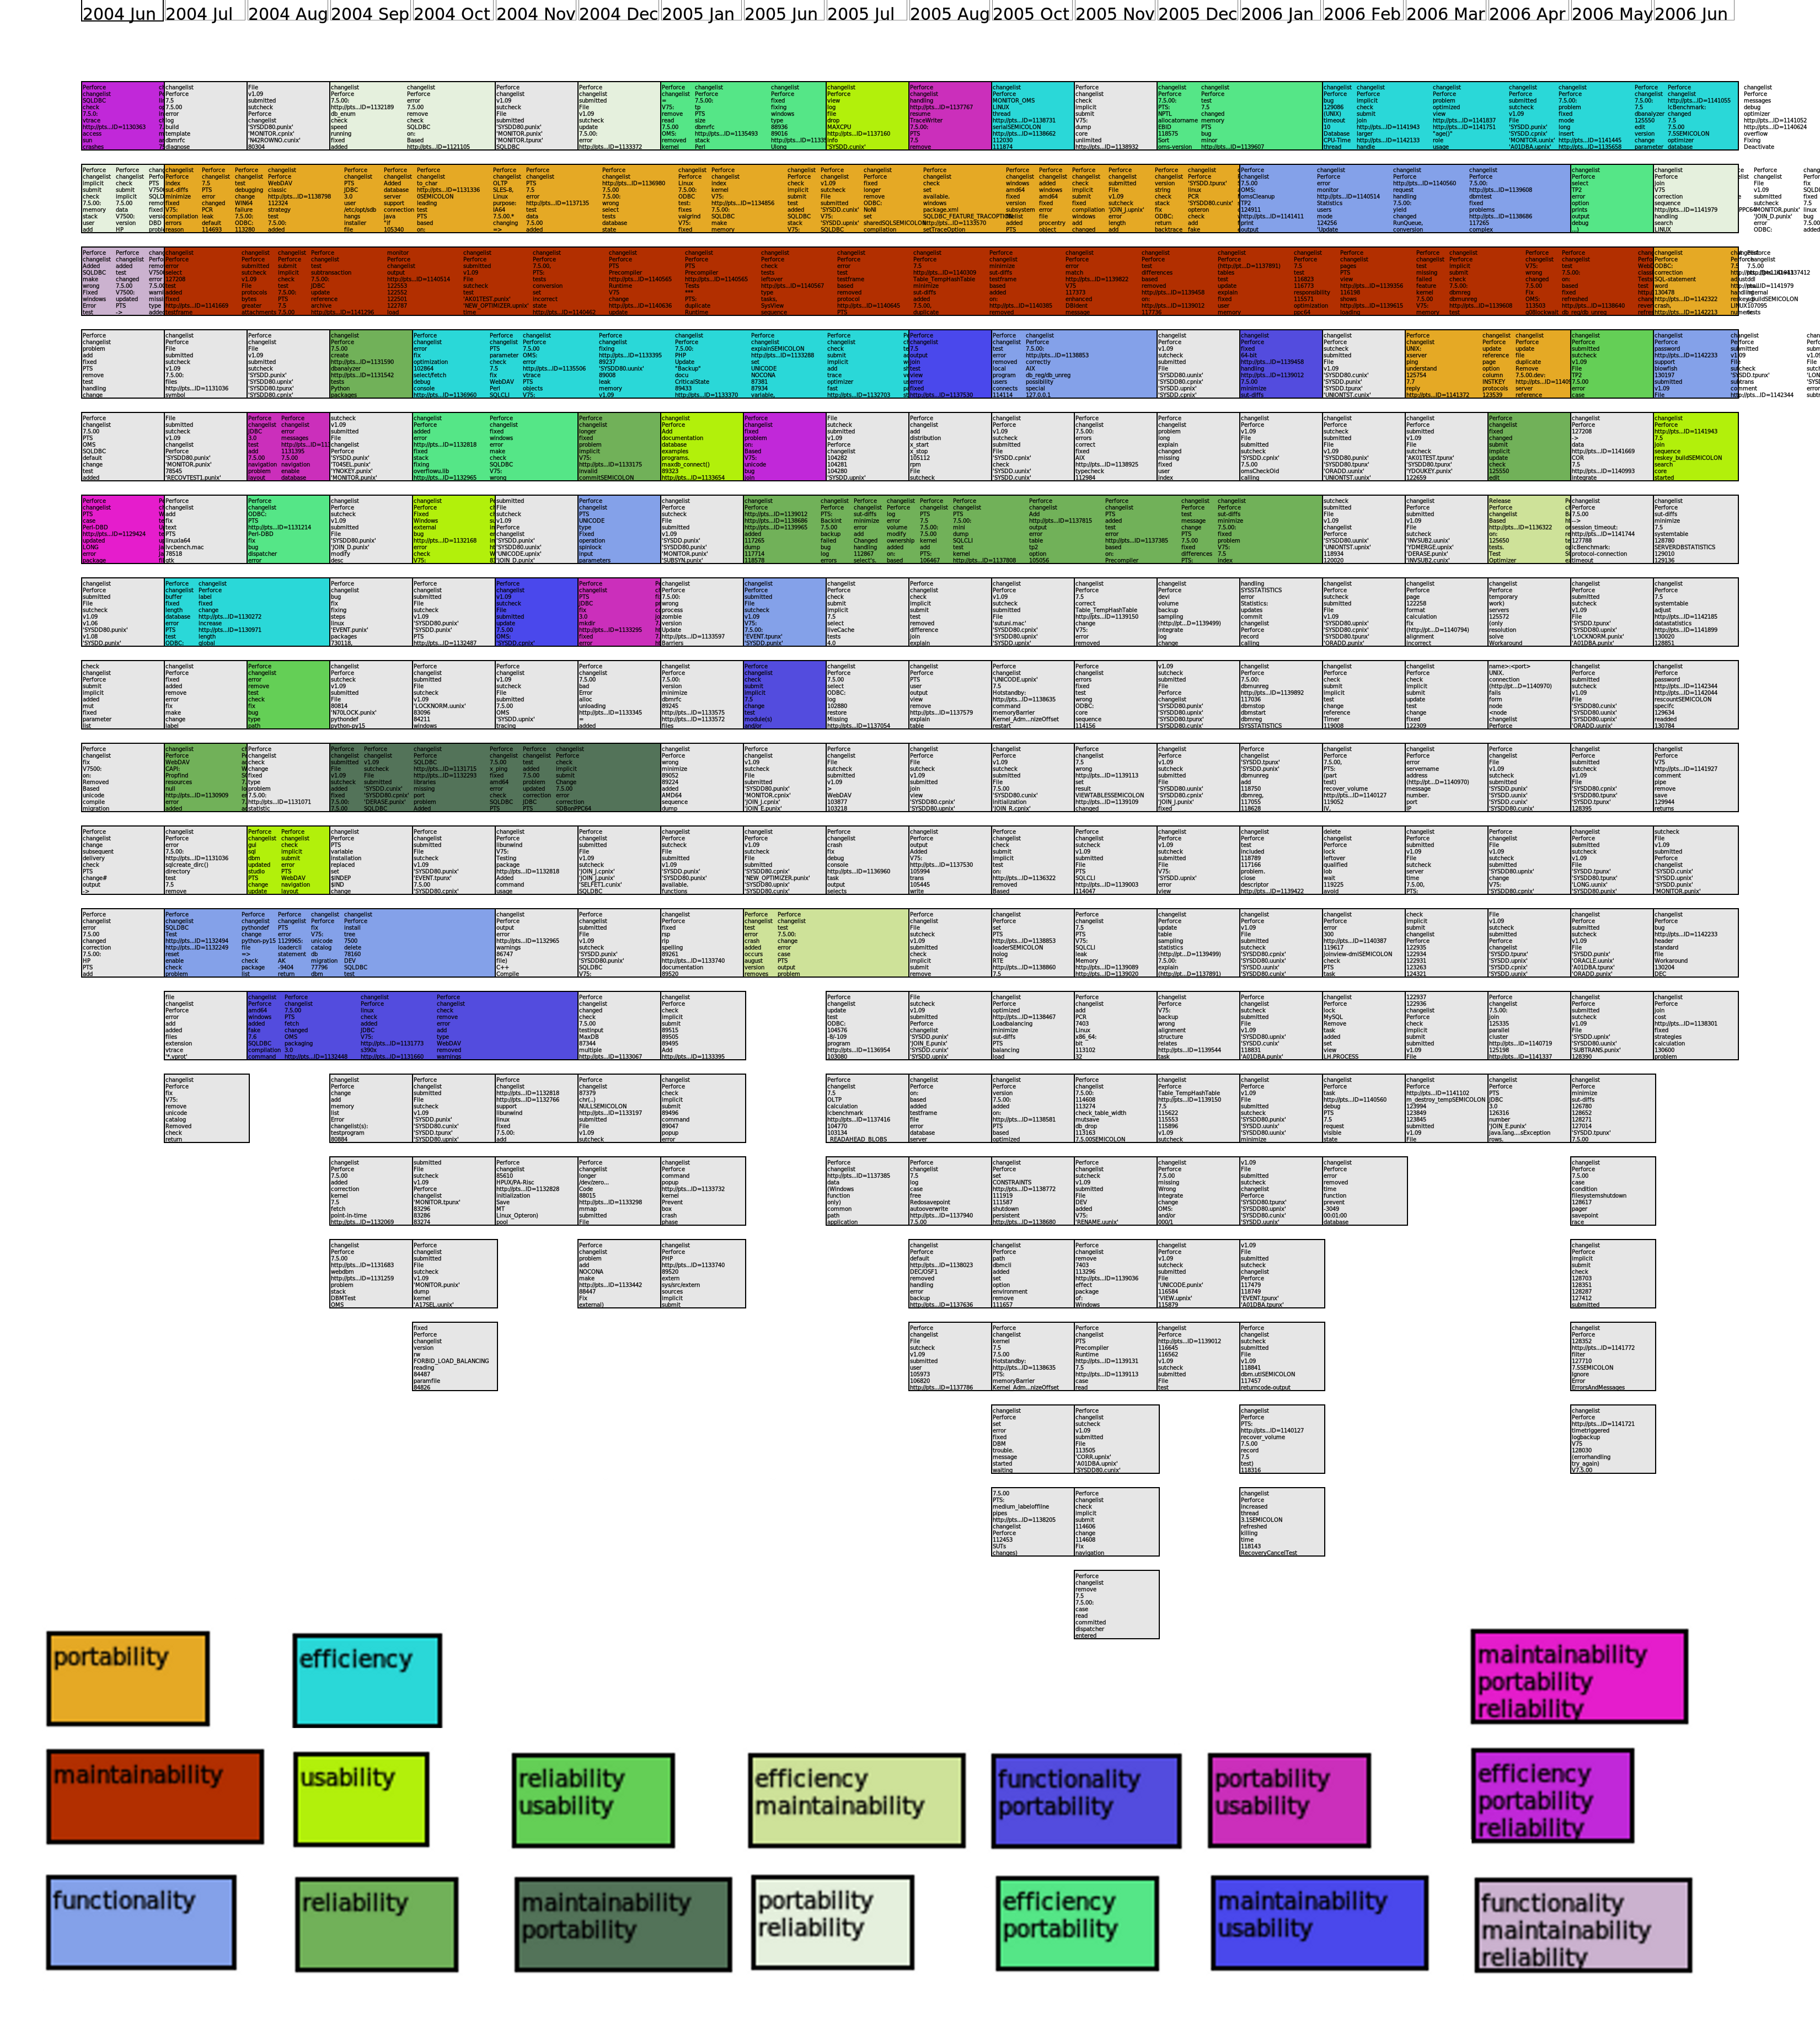
\includegraphics[height=.55\textheight]{maxdb-time-smear-plot-Equal}
  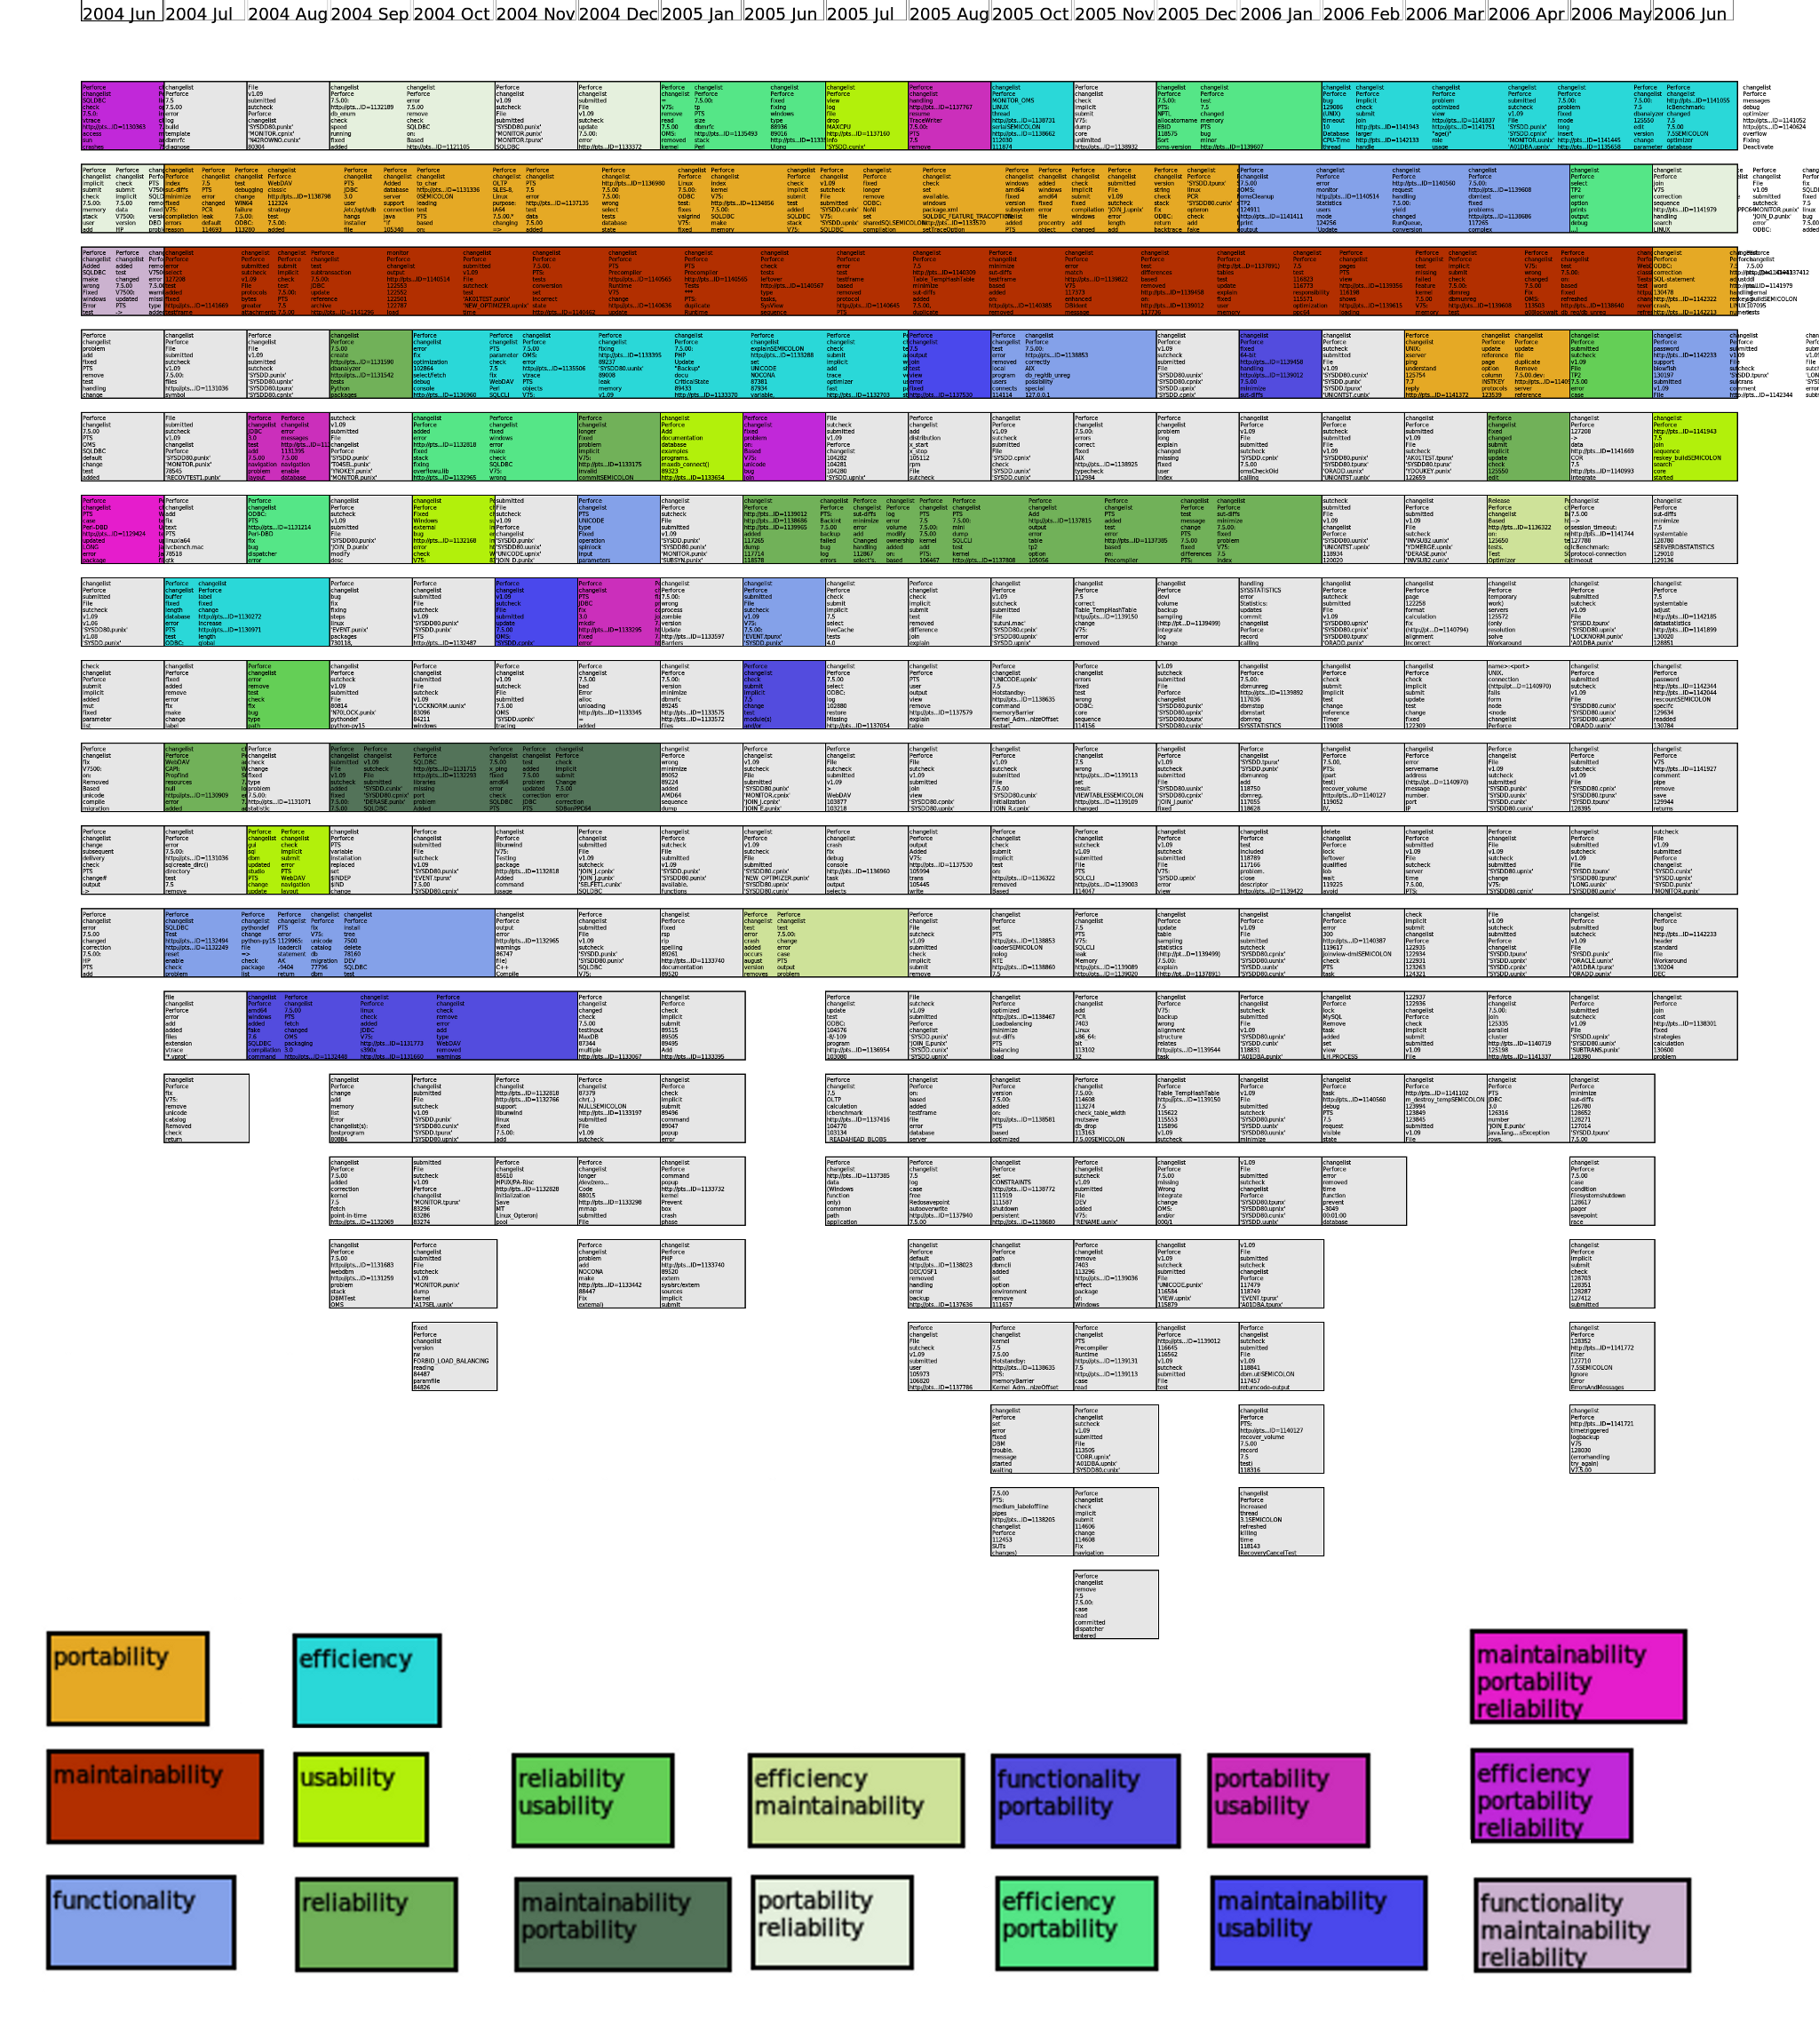
\includegraphics[height=.55\textheight]{small-maxdb-time-smear-plot-Equal}
  \caption{MaxDB 7.500: Labelled topics related to non-functional software qualities plotted over time, continuous topics are trends that occur across time}
  \label{fig:maxdb}
\end{figure*}

\begin{figure*}%[h]
  \centering
  % hi-res version
  % 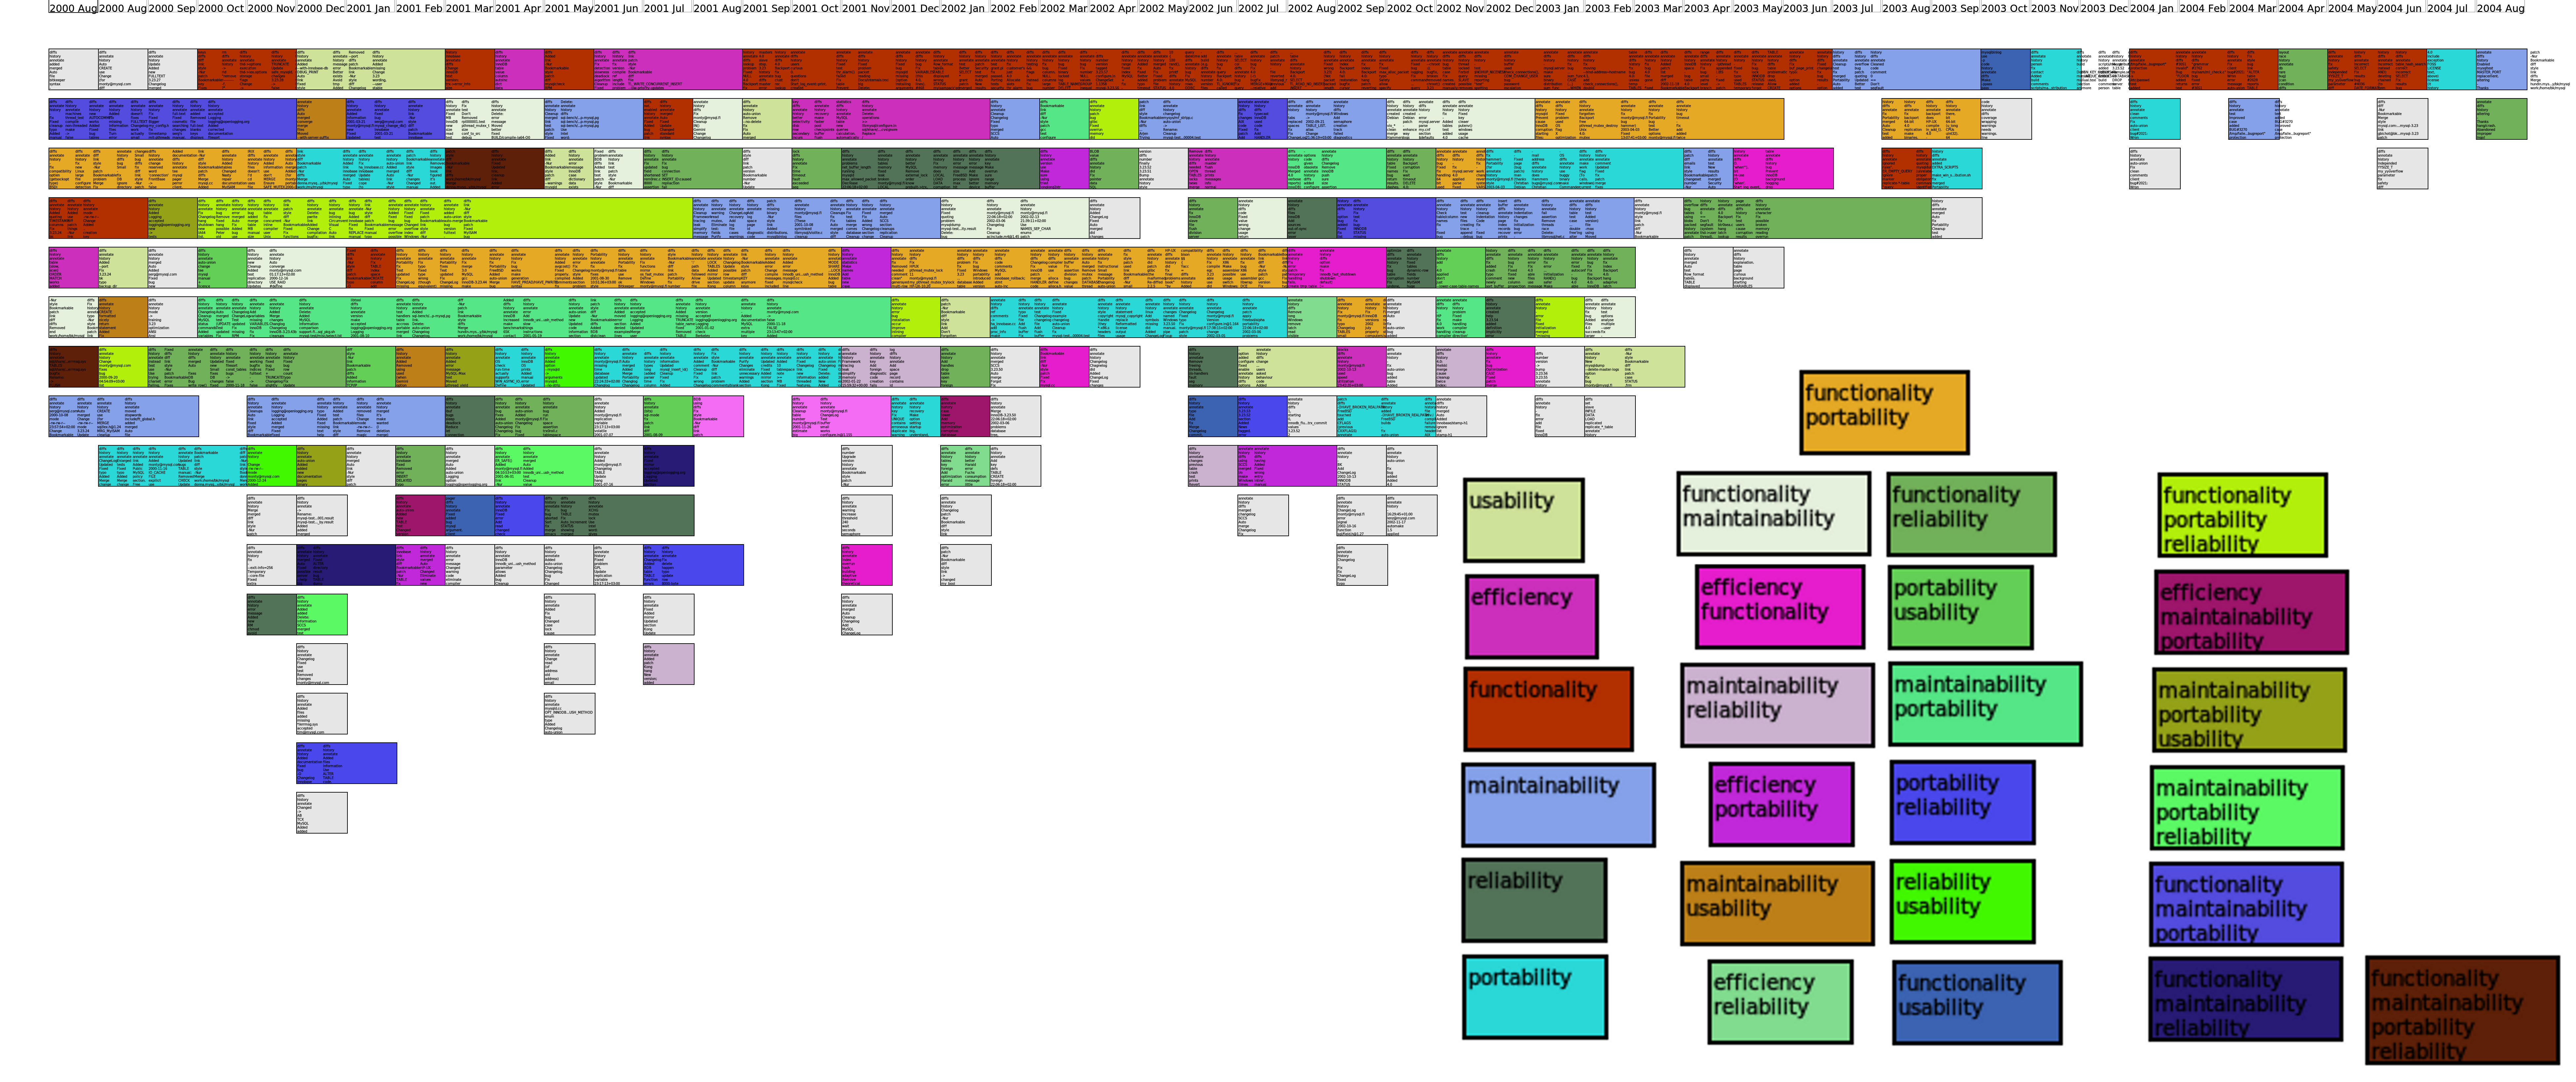
\includegraphics[width=.97\textwidth]{mysql-time-smear-plot-Equal}
  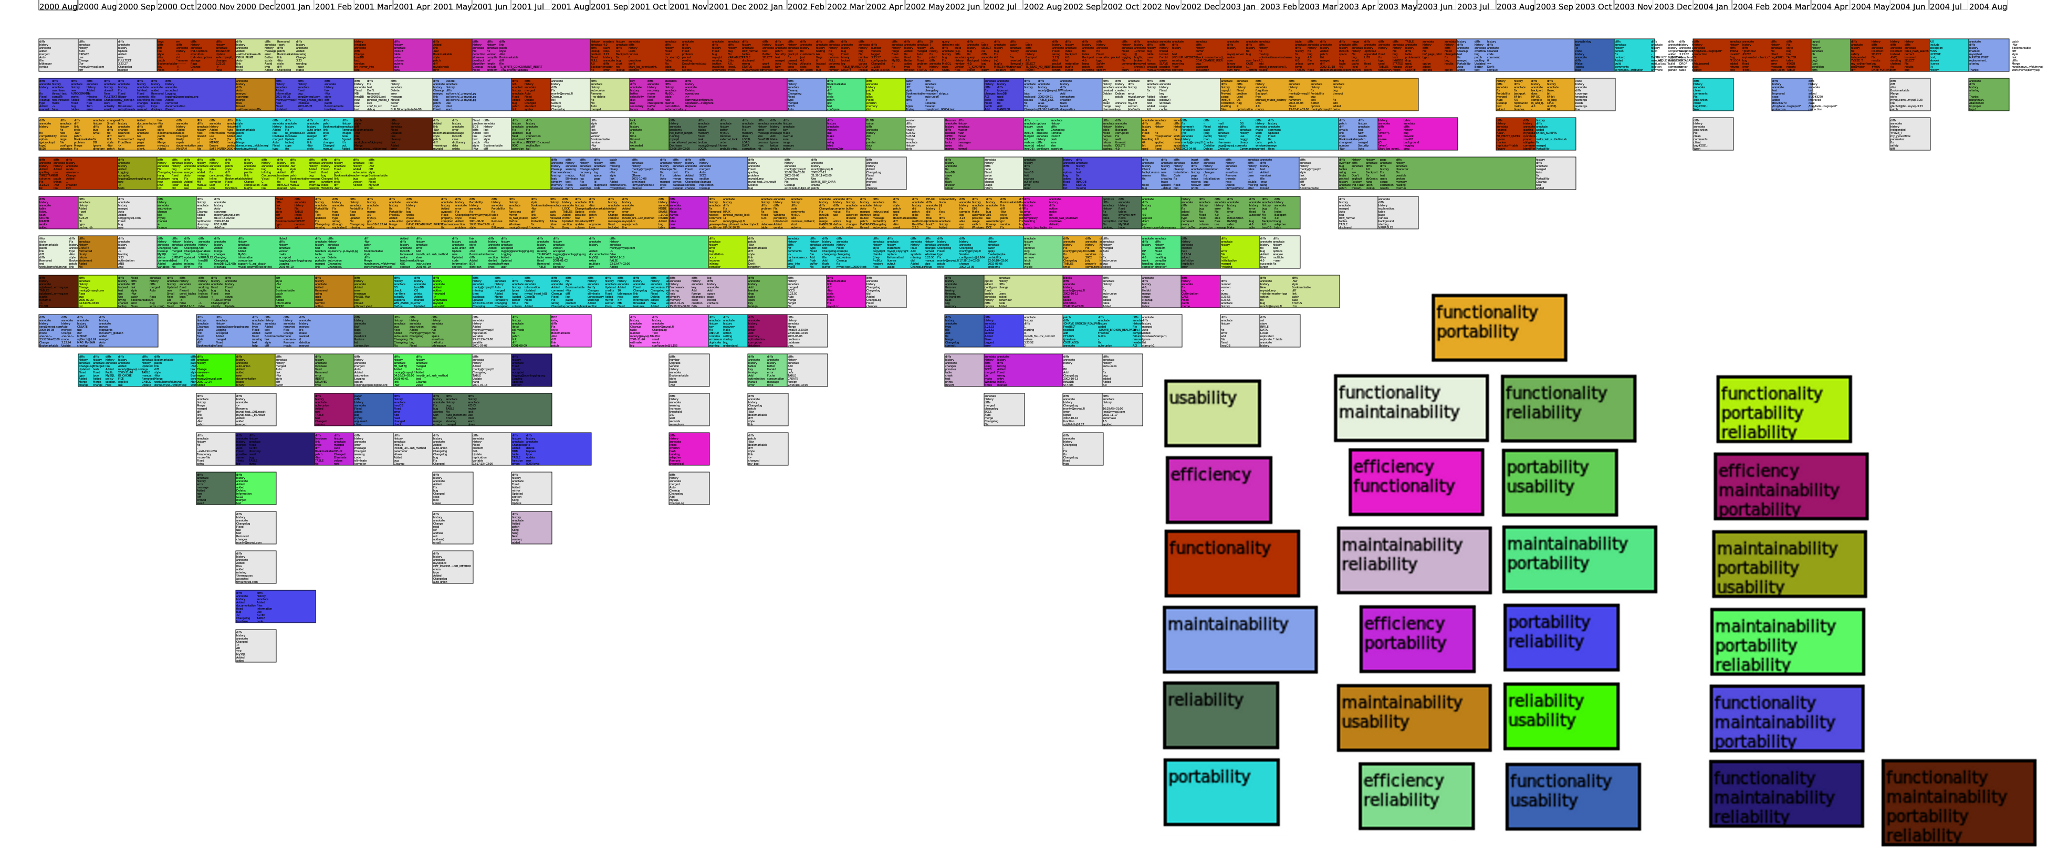
\includegraphics[width=.97\textwidth]{small-mysql-time-smear-plot-Equal}
  \caption{MySQL 3.23: Labelled topics related to non-functional software qualities plotted over time, continuous topics are trends that occur across time}
  \label{fig:mysql}
\end{figure*}


\shrink
\subsection{Comparing MaxDB and MySQL}

\label{sec:comparison}
%\XXX{Not sure there's enough here to do that!}

We observed that MySQL had more topic subsets than MaxDB. MySQL 3.23 also had more topics and a longer recorded history than MaxDB 7.500. We tagged more MySQL topics with annotations than MaxDB topics yet both shared similarities. In terms of non-functional requirements both projects had long running trends that focused on functionality, maintainability, and portability, yet MaxDB had more of a focus on efficiency and reliability. MaxDB differed from MySQL since MaxDB was being actively developed, whereas halfway through our history of MySQL 3.23, other versions of MySQL were being actively developed: MySQL versions 4.0, 4.1, and eventually 5.0 and 5.1. In other words, MySQL 3.23 was being maintained rather than actively developed, whereas MaxDB 7.500 was being actively developed into MaxDB 7.6, and then maintained thereafter.

MySQL and MaxDB's machine learners did make decisions based off some shared words. Words that were used to classify topics that were shared between MySQL and MaxDB included: \textsf{bug, code, compiler, database, HP UX, delete, memory, missing, problems, removed, add, added, changed, problem, and test}. Adding these words to the word bags of \textsf{exp2} and \textsf{exp3} could improve performance while ensuring they were only domain specific.

With respect to the questions raised in section \ref{sec:suplearn}:

\textbf{Do label frequencies change over time?} -- Yes, MySQL's label
frequencies decreased as it got older. Usability and reliability
labels became more and more infrequent as it matured. Maintainability topics
became more prevalent as MaxDB matured.

\textbf{Do the different projects differ in their relative topic
  interest?} -- Yes. MySQL 3.23 had proportionally more
functionality labelled topics, while MaxDB had proportionally more
efficiency and portability related topics.
 

\begin{comment}
 shared-report.sh ; cat output/shared-j48-words 

      2 bug
      2 code
      2 compiler
      2 database
      2 Delete_
      2 HP_UX
      2 memory
      2 missing
      2 monty_mysql_com
      2 monty_mysql_fi
      2 problems
      2 Removed
      2 work__home_bk_mysql
      4 4_0
      4 Add
      4 added
      4 Changed
      4 problem
      6 Added
      6 test

\end{comment}

\shrink
\subsection{Annotation observations}

We found many topics that were not non-functional requirements (NFRs) but were often related to them. For instance, concurrency was mentioned often in the commit logs and was related to correctness and reliability, because concurrency was troublesome. Configuration management and source control related changes appeared often and sometimes there were topics dedicated to configuration management. These kinds of changes are slightly related to maintainability. A non-functional change that was not quality-related was licensing and copyright; many changes were simply to do with updating copyrights or ensuring copyright or licenses headers were applied to files.

We noticed that occasionally the names of modules would conflict with words related to other non-functional requirements. For instance, optimizers are very common modules in database systems: both MySQL and MaxDB have optimizer modules. In MySQL the optimizer is mentioned but often the change deals with correctness or another quality. Despite this difference, the name of the module could fool our learners into believing the change was always about efficiency. Perhaps a project specific word-bag is needed in order to avoid automated mistakes due to the names of entities and modules with the software project.

\begin{comment}
A quick mind dump before I forget:
* portability was very popular
* there were many instances of concurrency
* There were often topics of crap commits with no comment
* might need more than the top words to compare
* Things like tests were noticable more by file type
* Configuration management is not part of the software quality ontology?
* I didn't tag none I tagged unknown, so that's some inconsistency between us
* There were a lot of copyright changes in mysql
* mysql had optimizer module which did not mean optimization
* I tried to assign reliability/bug for reliability bugs
  and Functionality/Correctness for fixes
* Some security changes came later
* Mysql 3.23 transitioned from a project being developed to
  a project being maintained, more frequent back-port bug-fixes
\end{comment}

\shrink
\subsection{Effectiveness}

%{Discuss how these are CHEAP techniques and although somewhat %inaccurate they don't require a tonne of work}

With ROC values ranging from $0.6$ to $0.8$ we can see there is promise in these attempts. \textsf{exp2} and \textsf{exp3} both indicate that static information can be used to help label topics without any training whatsoever. If the techniques used in \textsf{exp2} and \textsf{exp3} were combined with the supervised techniques we could probably reduce the training effort. 
Both Naive Bayesian learners and the word-list approaches were computationally efficient.  These results are promising, because the results are accurate enough to be useful, while still cheap enough to execute to be feasible as an automated or semi-automated method of labelling topics by their software qualities.

\shrink
\subsection{Threats to validity}

\begin{comment}
\textbf{Construct validity} -- Focus on code commit messages, rather than mail or bug trackers. Choice of taxonomy

\textbf{Internal validity} -- inter-rater reliability.

\textbf{External validity} -- Our data originated from open-source projects in the database domain. Of these, the open-source nature of the project seems most problematic for external validity. However, both projects are developed by commercial entities. Our technique is dependent on development practises including meaningful commit messages, which might not be true in other domains.
\end{comment}

Our study suffers from multiple threats to validity. \emph{Construct validity} issues include that we used only commit messages rather than mail or bug tracker messages. We also chose our taxonomy and the data to study. \emph{Internal validity} issues are to do with inter-rater reliability. \emph{External validity} issues are that our data originated from OSS database projects and thus might not be applicable to commercially developed software. Furthermore, our analysis techniques rely on a project's use of meaningful commit messages.

\shrink
\section{Related work}

\begin{comment}
% Part of our effort with this project is to understand the qualitative and intentional aspects of requirements in software evolution, a notion we first discussed in \cite{ernst07icsm}. That idea is derived from, in part, work on narratives of software systems shown in academic work from Ant\'{o}n et al.~\cite{anton01}, or more general-purpose work from Waldo~\cite{waldo93}.

% Part of our effort with this project is to understand the qualitative and intentional aspects of requirements in software evolution, a notion we first discussed in \cite{ernst07icsm}. That idea is derived from, in part, work on narratives of software systems shown in academic work like \cite{anton01}, or more general-purpose works like \cite{waldo93}. 


% Not sure how do handle this
\end{comment}
The idea of extracting higher-level `concerns' (also known as `concepts', `aspects' or `requirements') has been attacked in two ways. 

Cleland-Huang and her colleagues published work on mining requirements documents for non-functional requirements (NFR) (quality requirements)~\cite{Cleland-Huang2006}. One approach they tried was similar to this one, with keywords mined from NFR catalogues found in their previous work~\cite{chung99}. They managed recall of 80\% with precision of 57\% for the Security NFR, but could not find a reliable source of keywords for other NFRs. Instead, they developed a supervised classifier by using human experts to identify an NFR training set. There are several reasons we did not follow this route. One, we believe we have a more comprehensive set of terms due to the taxonomy we chose. Secondly, we wanted to compare across projects. Their technique was not compared across different projects and the applicability of the training set to different corpora is unclear. A common taxonomy allows us to make inter-project comparison (subject to the assumption that all projects conceive of these terms in the same way). Thirdly, while the objective of Cleland-Huang's study was to identify new NFRs (for system development) our study assumes these NFRs are latent in the textual documents of the project. Finally, the source text we use is less structured than their requirements documents.

In the same vein, Mockus and Votta~\cite{Mockus00} studied a large-scale industrial change-tracking system. They also leveraged WordNet, but only for word roots. They felt the synonyms would be non-specific and cause errors. A nice contribution was access to system developers, with whom they could validate their labels. Since we try to bridge different organizations, these interviews are infeasible (particularly in the distributed world of open-source software).

The other approach is to start with code repositories, and try to extract concerns from there. Marcus et al.~\cite{marcus04wcre} describe their use of Latent Semantic Indexing to identify commonly occurring concerns for software maintenance. Some results were interesting, but their precision was quite low. ConcernLines~\cite{treude09cl} shows tag occurrence using colour intensity. They mined change request tags (such as `milestone 3') and used these to make evolutionary analyses of a single product. The presence of a well-maintained set of tags is obviously essential to the success of this technique.

\begin{comment}
%We maintain that these results require more substantive manipulation before being reported to, for example, management. Like any large-scale data analysis project, it requires skill to derive the implications. Hooking the backend results directly to a reporting tool is unlikely to produce useful results.

% There has been an explosion of interest in mining OSS repositories. Godfrey and Tu \cite{godfrey00} were among the first to use this data to assess software evolution. They discussed how well the growth of Linux was predicted by laws that Lehman and colleagues \cite{lehman85} proposed. More recently, Herraiz et al. \cite{herraiz07icsm} predicted OSS growth using time series analysis. Like us, they refer to release windows as a useful unit of analysis. 
\end{comment}


Mens et al.~\cite{mens08icsm} conducted an empirical study of Eclipse, the open source software (OSS) source code editor, to verify the claims of Lehman~\cite{lehman97sms}. They concerned themselves with source code only, and found Law Seven, ``Declining Quality'', to be too difficult to assess: ``[we lacked an] appropriate measurement of the evolving quality of the system as perceived by the users \cite[p. 388]{mens08icsm}''. This paper examines the notions of quality in terms of a consistent ontology, as Mens et al. call for in their conclusions.

Mei et al.~\cite{Mei2007} use context information to automatically name topics. They describe probabilistic labelling, using the frequency distribution of words in a topic to create a meaningful phrase. They do not use external domain-specific information as we do.
In \cite{ernst10refsq}, we describe our earlier project, similar to this, to identify change in quality requirements in GNOME software projects; our approach is solely text-matching, however, and does not leverage machine learning strategies.

\begin{comment}
% comment out or not
% Massey~\cite{massey02icse} and Scacchi~\cite{scacchi02,scacchi05b} looked at the topic of requirements in open-source software. Their work discusses the source of the requirements and how they are used in the development process. German~\cite{german03gnome} looked at GNOME specifically, and listed several sources for requirements: leader interest, mimicry, brainstorming, and prototypes. None of this work  addressed quality requirements in OSS, nor did it examine requirements trends.

% Hindle et al. \cite{Hindle2007} examined release patterns in OSS. They showed that there is a difference between projects regarding maintenance techniques. This supports our result that software qualities are not discussed with the same frequency across projects.
\end{comment}

% Most of this related research examined project source code. Software mining of other project corpora is less common. Similarities exist with approaches that begin with structured taxonomies, as with the Hismo software ontology~\cite{girba06}. Rigby and Hassan~\cite{rigby07msr} used a general purpose taxonomy to classify developer email according to temperament.

\shrink
\section{Conclusions and future work}

We demonstrated that static but domain-specific knowledge can improve unsupervised labelling of extracted topics. Our \textsf{exp2} experiment used small accurate word bags to label topics but performed just as well as \textsf{exp3}, which used many more general terms from WordNet. We then showed that with some supervision, and by using efficient machine learners based on Naive Bayesian classifiers, we could improve the accuracy of automatic labelling topics even further.

Our manual inspection and annotation of the topics extracted from MySQL and MaxDB revealed that many of the extracted topics dealt with non-functional requirements, and these topics were spread across the entire history of a project. In the cases of MaxDB and MySQL, portability was a constant maintenance concern and was prevalent throughout the entire lifetime of the projects.

We showed that non-functional requirements are often trending topics, that non-functional requirements are quite common in developer topics, and that there are efficient methods of semi-automating and automating topic labelling.

There are many avenues of further investigation.  We want to investigate developer attitudes related to these labels: i.e., when we label a topic, was the developer expressing positive or negative qualities about that label?  It is difficult to map abstract qualities to particular messages. Is a ``quality'' discussion about more than just corrective maintenance? %In this study we take the position that any type of maintenance has to do with software quality.

%\section{Acknowledgements and appendix}
Our data and scripts are available at \url{http://softwareprocess.es/nomen/}

\bibliographystyle{abbrv}
%\bibliographystyle{IEEEtran}
\bibliography{icpc}

\end{document}

